\chapter{Bulk medium evolution and initial condition}
In this chapter, I shall introduce a hydrodynamic based model for describing the bulk medium evolution in the heavy-ion collision.
After the basic description of the modeling, I will show an application of this simulation framework in reverse engineering the three-dimensional initial entropy deposition, which is one of my published research projects.

\section{A Hydrodynamics-based dynamical modeling}
\subsection{The hydrodynamic equations}
There has been vast experimental evidences that supports the use of an relativistic viscous hydrodynamics in describing the dynamical evolution of the medium created in the heavy-ion collision.
At mid-rapidity, the hydrodynamic-based model can achieve a high precision of agreement with a global comparison to experimental data. 
This data also support the use of a small but nonzero specific shearviscosity {Muronga:2004sf, Chaudhuri:2006jd, Romatschke:2007mq, Dusling:2007gi, Song:2007ux, Luzum:2008cw}, and more recent studies and global Bayesian analysis also suggest the use of a finite bulk viscosity.

\paragraph{Ideal hydrodynamics} Hydrodynamics is a macroscopic description that propagates the energy momentum tensor of the system without an microscopic knowledge of the degrees of freedom.
The first four equations comes from the the energy-momentum conservation,
\begin{eqnarray}
\partial_\mu T^{\mu\nu} = 0
\end{eqnarray}
where $T^{\mu\nu}$ is the energy momentum tensor and $\partial_\mu = \partial/\partial x^\mu$. 
Here we have choose the metric as $g^{\mu\nu} = \diag\{1, -1, -1, -1\}$.
If one assumes ideal hydrodynamics that the system always relax to local thermal equilibrium fast enough compared to other time scale, then $T^{\mu\nu}$ can be expressed as
\begin{eqnarray}
\partial_\mu T^{\mu\nu} = e u^\mu \nu - P (g^{\mu\nu}-u^{\mu\nu})
\end{eqnarray}
where $u^\mu$ is the flow velocity such that in the co-moving frame  $T^{\mu\nu}$ has the diagonal form $T^{\mu\nu} = \diag\{e, -P, -P, -P\}$.
Therefore $e$ and $P$ are the energy density and pressure of the thermalized matter in the rest frame.
There are five unknowns $e, P, u_x, u_y, u_z$ ($u_t$ is determined by $u^2 = 1$), but conservation laws only provide four equations.
A fifth equation is the equation of state (EoS) $P = P(e)$ that encodes thermodynamic properties of the medium (in this case, the nuclear medium at finite temperature) which closes the set of ideal-hydrodynamic equation.
\paragraph{Inputs from first principal calculation} The lattice QCD simulation has determined the QCD equation of state to high precision with physical masses of the light flavor.
It is not a prior known that the lattice QCD EoS computed for an infinite matter in infinite time is the best choice for describing a transient, finite size system, however, using the lattice input does result in reasonable agreement with the data.
Moreover, there has been a study that try to constrain the from of EoS from experimental data and the ``calibrated'' EoS is very close the Lattice prediction.
Most of the currently hydrodynamic studies already uses the state-of-the-art lattice results.
\paragraph{Viscosity correction and QCD transport coefficient}
The medium created in heavy-ion collision undergoes fast longitudinal and transverse expansion, and the thermalization rate may not be fast enough to keep the system in fully thermal equilibrium,
\begin{eqnarray}
T^{\mu\nu} = u^\mu u^\nu e - (g^{\mu\nu}- u^\mu u^\nu) (P+\Pi) + \pi^{\mu\nu}
\end{eqnarray}
Here $T_0$ is the thermal part, and $\pi$ is the shear viscosity correction, and $\Pi$ is the bulk viscosity correction to the pressure.
Relativistic viscosity hydrodynamics that expands the transport description in terms of the Knudsen number is developed to taken into account viscous effects.
At first order, this is well-known Naiver-Stokes equations, where the $\pi$, $\Pi$ are given by the constitutive relations,
\begin{eqnarray}
\pi^{\mu\nu} &=& 2\eta\sigma^{\mu\nu}\\
\Pi &=& -\zeta\theta
\end{eqnarray}
Here the corrections to the energy momentum tensor are proportional to the first gradient of the macroscopic field $\sigma^{\mu\nu} = \partial^{\langle \mu} u^{\nu\rangle}, \theta = \partial\cdot u$.
The proportional constant are known as the (first order) transport coefficient of the QCD matter, which encodes the dynamical information of the system. 
Especially their dimensionless ratio to the entropy density $\eta/s$ and $\zeta/s$ are important indicator of the interaction strength and the scale-violation of the QCD matter and are of great physical importance.
There have been many effort to either computing these quantities from first principles and effective models or extracting these numbers in a model-to-data comparison.
Coming back to the hydrodynamic modeling, it is shown that one has to go to second order in the expansion to the render the correction compatible with special relativity and $\pi$, $\Pi$ becomes dynamical quantities which tends to relax to the Naiver-Stokes limit.
\begin{eqnarray}
\nonumber
\tau_\pi \dot{\pi}^{\langle\mu\nu\rangle}+\pi^{\mu\nu} &=& 2\eta\sigma^{\mu\nu}- \delta_{\pi\pi}\pi^{\mu\nu}\theta + \phi_7 \pi_{\alpha}^{\langle\mu}\pi^{\nu\rangle\alpha}-\tau_{\pi\pi}\pi_{\alpha}^{\langle\mu}\sigma^{\nu\rangle\alpha} + \lambda_{\pi\Pi}\Pi\sigma^{\mu\nu},
\\
\nonumber
\tau_{\Pi}\dot{\Pi} + \Pi &=& -\zeta\theta - \delta_{\Pi\Pi}\Pi\theta + \lambda_{\Pi\pi}\pi^{\mu\nu}\sigma_{\mu\nu}.
\end{eqnarray}
The $\delta, \phi, \lambda$ are known as second order transport coefficients.
This complicated set of equations together with the conservation law and the EoS forms the viscosity hydrodynamic equations.
Nowadays, well tested numerical packages have been developed solving these equations in the context of heavy-ion collisions.

\paragraph{Boost-invariance approximation and beyond}
In general, the hydrodynamic equations have to be solved as a 3+1 dimensional problem.
But a reduction to a 2+1 dimension is possible, if one assume the fast expansion along the beam-axis (longitudinal) direction has an approximated symmetry near mid-rapidity.
This approximate symmetry is first proposed by Bjorken in [] that the system at different rapidity looks similar upto a longitudinal boost, so that one may first obtain the solution to the 2+1 dimension problem at one space-time rapidity ($\eta_s = 0$) and then boost the solution to other $\eta_s$.
A direct consequences of this symmetry is that the observables should not depends on space-time rapidity.
The $\eta_s$-dependence cannot be directly detected, but can be related to the the rapidity / pseudo-rapidity for the reason below.
Suppose that the Lorentz contracted nuclei interact at $z=0$ and produce excitations that free-stream in the longitudinal direction, then for each of these excitation
\begin{equation}
  \frac{z}{t} = \frac{p_z}{E}.
\end{equation}
This approximation the equivalence of $\eta_s$ and $y$ at early stages of the collision:
\begin{equation}
  \eta_s = \frac{1}{2}\log\frac{t+z}{t-z} \sim y = \frac{1}{2}\log\frac{E+p_z}{E-p_z}.
\end{equation}
If one further assumes these initial excitations are mass-less partons, then the rapidity can be approximated by pseudorapidity as $E\approx |p|$.
The event-averaged rapidity-distribution of charged particles $dN_{\textrm{ch}}/dy$ in both proton-proton and symmetric nuclei-nuclei collisions at the LHC energy falls at large rapidity but has a slowly varying profile at mid-rapidity within $|y|<2$, which is a motivation to apply the boost-invariant at mid-rapidity as a first approximation.

However, since $dN_{\textrm{ch}}/dy$ are event-averaged quantities, its being flat within $|y|<2$ does not rule out that event-by-event particle production fluctuation can break the approximation, and these fluctuations, local in transverse plane, can be different at different transverse location.
Moreover, asymmetric nuclear collision such as $p+Pb, p+Au, d+Au, He+Au$, etc clearly breaks the boost-invariance even on an event averaged level. 
Therefore, the study of longitudinal fluctuation related observables or the search for hydrodynamic  behavior in small collision system clearly requires one to go beyond the boost-invariance approximation.

\subsection{Particularization and microscopic transport}
The longitudinal expansion and the transverse expansion driven by the pressure difference cools down the system temperature and density rapidly and eventually the relaxation rate is too low for the the hydrodynamic approach to apply.
When this happens, one can switch to the microscopic transport description of the system.
This switching is usually done near or below the pseudo-critical temperature $T_{sw} \lesssim T_c$ so that the energy momentum tensor can be particularized as an ensemble of hadrons .
This choice $T_{sw} \lesssim T_c$ avoids the problem of modeling quark / gluon dynamics and hadronization in the strong coupled regime near $T_c$, and whether a hydrodynamics with lattice EoS and a hadronic transport model with cross-sections as inputs are both valid in this regime is another question.
The hydrodynamic $T^{\mu\nu}$ is usually particlized at a constant energy density / temperature hypersurface using the Cooper-Frye formula,
\begin{eqnarray}
dN_i^a(p) = \frac{g^a f^a(p) dp^3}{(2\pi)^3}  \frac{p^{\mu}}{E} \Delta \sigma_{i,\mu} 
\end{eqnarray}
Where the particle yield of specie ``$a$'' with momentum $p$ from the $i^{\textrm{th}}$ surface element $\sigma_{i,\mu}$ equals its phase space density times the surface area (with units of a 3D volume) parallel to the  four velocity $p^\mu/E$.
This distribution function should include both a thermal part and a viscous correction, $f = f_0 + \delta f$.
There are more than one way to construct the viscous correction $\delta f$  from $e, P, n, \Pi$ and $\pi^{\mu\nu}$ based on different assumptions of the form of corrections.
In this work, we shall use a non-additive $\delta f$ correction that has been developed and implemented by [] and [], and please refer to the references for the original formulation and numerical implementations details.

The particlized hadronic system is then solved by the Ultra-relativistic Quantum Molecular Dynamics (UrQMD) model until the system is dilute enough and interactions ceases (kinetic freezeout). 
The UrQMD in the context of hadronic cascade (afterburner) includes processes like resonance decays, elastic and inelastic scatterings, and string formations and fragmentations.

\subsection{Pre-equilibrium stage}
At very early times of the collision, the system is off equilibrium. 
However, viscous hydrodynamic assumes a closeness to the local thermal equilibrium  (there are also recent efforts in studying the effectiveness of hydrodynamics outside of its traditional range of application []).
A successful prediction using an early onset of hydrodynamic evolution at $\tau_0\lesssim 1$fm/$c$ suggests a fast hydrodynamization, whose exact mechanism is still a debatable question. 
There are different modelings of this pre-equilibrium stage, including solving the classical Yang-Mills equation [], partonic transport models [], a collision-less Boltzmann equation [], and the linear response method of the effective kinetic approach [].

Such a pre-equilibrium stage was not included in my study of the 3D initial condition, where the simulation starts at $\tau_0 = 0.6$ fm/$c$ assuming local thermal equilibrium.
For my later study of the heavy flavor dynamics, a 2+1D collision-less Boltzmann equation implemented by [] was later used in obtaining the medium evolution history.
In such a model, the initial energy density ($\tau = 0^+$) at mid-rapidity  is thought to be carried by mass-less partons that propagates at the speed of light in the transverse direction. 
The initial distribution function is assumed to have a factorized form $f(x_\perp, p_\perp, \tau=0) = n(x, \tau=0) \times dN/dp_\perp^2$.
The momentum distribution $dN/dp_\perp^2$ do not evolve as the collisions are neglected, while the spatial density evolves as
\begin{eqnarray}
n(\vec{x}, \tau) = \int n(\vec{x}', \tau=0) \delta^{(2)}(\vec{x} - \vec{x}'- \tau) d\vec{x}'^2
\end{eqnarray}
Then, the model assumes a sudden hydrodynamization at time $\tau_{\textrm{hydro}}$, where the free-streamed,
\begin{eqnarray}
T^{\mu\nu}(x_\perp, \tau_{\textrm{hydro}}) = \int f(x_\perp, p_\perp, \tau=0) \frac{p^\mu p^\nu}{E} dp^3
\end{eqnarray}
is used for initializing the hydrodynamic equations by the Landau matching procedure [].

\section{Initial condition model}
Unlike the dynamical models that are governed by a few equations / laws with a few parameters, the initial condition model parameterizes many more unknowns.
For different initial condition models, these unknowns can be initial color density of the nuclear wave function, the effective size of a nucleon, the form factor of nucleon-nucleon inelastic cross-section, and the amount of fluctuations in particle production / energy deposition, etc.
There are two classes of initial condition models:
\begin{itemize}
\item Models that takes into the particle production dynamics. Such as minijet production, strings productions and flux-tubes, hadronic transport,and color-glass condensate (CGC) effective field theory based models {Wang:1991hta, Zhang:1999bd, Werner:2010aa, Petersen:2008dd, Schenke:2016ksl, Dumitru:2011wq, Hirano:2012kj}.
\item Parametric models that provides macroscopic initial conditions without a dynamical component. Such as Monte-Carlo Glauber models and its extensions [Bozek:2015bna], and the \trento model to be explained [Scott].
\end{itemize}
I shall focus on the development of a parametric model \trento to help the understanding of the initial three-dimensional entropy deposition.


\subsection{The original (boost-invariant) \trento\ model}
The original \trento\ model is proposed as a flexible ansatz to investigate a family of entropy / energy deposition behaviors at mid-rapidity.

First, the impact parameter $\vec{b}_{AB}$ between the two colliding nuclei $A$ and $B$ is sampled at random.
Then, the 3D nucleons positions inside each nuclei are sampled according to the Woods-Saxon distribution (for heavy nuclei, for light nuclei such as Deuteron, Helium, Oxygen where the nucleon distribution is not well approximated by a Woods-Saxon form, the sampling are different),
\begin{eqnarray}
\frac{df_N}{r^2 dr d\phi d\cos\theta} = \frac{1}{\exp\{\frac{r-R(1+\beta_2 Y_{20}(\theta)+\beta_4 Y_{40}(\theta))}{a}\}+1}
\end{eqnarray}
including the quadrupole and hexadecapole deformation of certain nuclei.
The randomized nucleon position is critical to explain the odd order of flow harmonics observed in experiments [].

Then, the collision between the two nuclei is analyzed at the nucleon level. 
Every nucleon pair $\{i, j\}$ with $i$ from nuclei $A$ and $j$ from nuclei $B$ has a certainty probability to undergo an inelastic collision, given the impact parameter $\vec{b} = \vec{b}_{AB} + \vec{x}_{i, \perp} -  \vec{x}_{j, \perp}$,
\begin{eqnarray}
P(b; \sigma) = 1 - \exp\left[-\sigma T_{pp}(b)\right],
\label{dsigma_db}
\end{eqnarray}
where $T_{pp}(b)$ is the overlapping function between the density of the nucleon,
\begin{eqnarray}
T_{pp}(b) = \int d\vec{x}_\perp^2 T_p(\vec{x}_\perp-\vec{b}/2) T_p(\vec{x}_\perp+\vec{b}/2)
\end{eqnarray}
And each nucleon is assumed to have a Gaussian density profile, 
\begin{eqnarray}
T_p(\vec{x}_\perp^2) = \frac{1}{2\pi w^2} \exp\left(-\frac{\vec{x}^2}{2w^2}\right)
\end{eqnarray}
with the width of the nucleon $w$ a free parameter.
The $\sigma$ is an effective constituent cross-section that is determined by reproducing the experimental measured proton-proton inelastic cross-section at a given beam energy,
\begin{eqnarray}
\sigma_{pp}^\text{inel}(\sqrt{s}) = \int d\vec{b}^2 P(b; \sigma(\sqrt{s}))
\end{eqnarray}
Applying the probabilistic collision criteria of equation \ref{dsigma_db} to each pair of nucleons, the nucleons that suffer at least one inelastic collisions are called participant and the total number of binary inelastic collisions are denoted as $N_{\textrm{bin}}$.
The minimum-biased event sample in the \trento model are defined all events that has at least one binary collision, 

The above procedure is similar to the that of an Monte-Carlo Glauber model in determine the nuclear inelastic cross-section.
The key step of \trento is an ansatz that maps from the participants in a particular event to the energy / entropy density deposited at the mid-rapidity.
We fist define the participant densities,
\begin{equation}
T_{A, B}(\x) = \sum_{i\in \textrm{Parts}_{A, B}} w_i\, T_p(\x - \x_i).
\end{equation}
The summation goes over the participants in nuclei $A$ and $B$, and each participant contribute a fluctuating contribution proportional to its transverse density $T_p$.
The fluctuating weight $w_i$ follows a $\Gamma$-distribution with unit mean and variance $1/k$ where $k$ is a parameter.
This fluctuating contribution is put in to mimic the multiplicity fluctuation in the proton proton collisions.
The entropy / energy density deposit at mid-rapidity is assumed to be a function of $T_A$ and $T_B$ only at each transverse location,
\begin{eqnarray}
\frac{dS(\vec{x})}{d\eta dx_\perp^2} \textrm{ or } \frac{dE(\vec{x})}{d\eta dx_\perp^2} = f(T_A(\vec{x}), T_B(\vec{x})).
\end{eqnarray}
This simplification is possible because at $\tau=0^+$, causality requires that the entropy production at one location cannot be correlated with the information at a different transverse location. 
Also, the partons that contribute to the bulk low-$p_T$ particle production at high $\sqrt{s}$ are predominately low energy gluons whose longitudinal wavelength is longer than the contracted proton radius in the $z$-direction; therefore, the entropy production should not be sensitive to the details of how the participants aligned but only its $z$-integrated density.
\trento\ parametrizes this mapping from $T_A$ and $T_B$ to the energy / entropy deposition using a ``generally mean'' ansatz,
\begin{eqnarray}
f(T_A, T_B; p) = \left(\frac{T_A^p + T_B^p}{2}\right)^{1/p}.
\end{eqnarray}
$p$ is a tunable parameter and with a few special values, it reduces to the well known average procedures as in table \ref{tab:trento-p}
\begin{table}
\centering
\caption{\trento\ $p$-parameter}\label{tab:trento-p}
\begin{tabular}{ccc}
\hline
$p\in \mathbb{R}$ & $f(x, y)$ & Entropy / energy production\\
\hline
$-\infty$ & $\min\{x, y\}$ &  dominated by the thinner target\\
$-1$ & $2xy/(x+y)$ &   the harmonic mean scaling\\
$0$ & $\sqrt{xy}$ &  the geometric mean scaling\\
$1$ & $(x+y)/2$ &  the arithmetic mean (participant) scaling\\
$+\infty$ & $\max\{x, y\}$ &  dominated by the thicker target \\
\hline
\end{tabular}
\end{table}
This way the model is able to parametrize a class of entropy / energy production scheme and includes certain type of initial condition uncertainty.
Through a global model-to-data comparison, this $p$ parameter has been calibrated to be very close to 0, suggesting the data favors a mid-rapidity entropy / energy deposition that scales as $(T_A T_B)^{0.5}$.
A similar scaling is also found in the EKRT initial condition model based on pQCD plus saturation physics.

\subsection{Parametrize the longitudinal dependence in \trento}
The \trento\ model has been doing successful phenomenology for obserables at mid-rapidity [].
My later work focus on extending the parametrization to a rapidity-dependent initial condition, and seek for a reverse-engineered 3D entropy production from the rapidity-dependent observables.

One constrain in extending the model is that it should reduces to the boost-invariant version of the model at mid-rapidity; therefore, I take the following decomposition of $s(\x, \eta_s)$ at the hydrodynamic starting time $\tau_0 = 0.6$ fm/c,
\begin{equation}
  s(\x, \eta_s)\vert_{\tau=\tau_0} \propto f(T_A(\x), T_B(\x)) \times g(T_A(\x), T_B(\x), \eta_s),
  \label{factorized}
\end{equation}
$f$ is the entropy production at midrapidity as explain above.
Now $g$ parametrize the rapidity-dependence and is always normalized such that $g(T_A(\x), T_B(\x)), 0)=1$.
Qualitatively, the breaking of boost-invariance can come from the initial asymmetry of the incoming nuclear matter $T_A \neq T_B$ and various sources of fluctuation in particle production.
We listed the sources of these contributions and indicated what contribution has been included and what is not,
\begin{itemize}
\item In asymmetric collisions like $p$-$A$ and non-central $A$-$A$, the local thickness functions are imbalanced $T_A \neq T_B$.
\item Even in central $A$-$A$ collision, nuclear / nucleon configuration fluctuations also contribute to the asymmetry. These are included as the randomized nucleon position fluctuation and the $\gamma$-fluctuation of the nucleon thickness function.
\item Initial stage dynamical evolution which can introduce dynamical fluctuations and non-vanishing flow in the $z$-direction is not included.
\end{itemize}
Therefore, the asymmetry in the extended \trento\ model only comes from the imbalanced and fluctuating participant density function.
We parametrize this function in terms of rapidity and then transformed to the space-time rapidity.
\begin{eqnarray}
g(\x, \eta) &=& g(y; T_A(\x), T_B(\x)) \frac{J \cosh \eta_s}{\sqrt{1 + J^2 \sinh^2 \eta_s}},
\label{jacobian}
\end{eqnarray}
where the species-dependent factor $J$ is replaced with an effective value $J \approx \langle p_T \rangle / \langle m_T \rangle$.
Instead of determining a single number at mid-rapidity, we need to map $T_A$ and $T_B$ to a function $g(y; T_A(\x), T_B(\x))$ that has infinite degrees of freedom.
To do these, we choose to parametrize how the $y$-cumulents of $g$ changes with $T_A$ and $T_B$, and reconstruct the function using its first few cumulants (mean $\mu$, standard deviation $\sigma$, and skewness $\gamma$)
\begin{eqnarray}
g(\x, y) &=& \mathcal{F}^{-1}\{\tilde{g}(\x, k)\}, \\
\log \tilde{g} &=&  i \mu k - \frac{1}{2}\sigma^2 k^2 - \frac{1}{6} i \gamma \sigma^3 k^3  e^{-\frac{1}{2}\sigma^2 k^2} + \cdots \label{cgf}
\end{eqnarray}
where for the skewness term, we have included an exponential that systematically includes higher order cumulants to regulate the behavior of the function at large $y$.
Numerically, we have found that within the range of $|y| < 3.3\sigma$, the reconstructed function has a good behavior and remains positive definite.

The remaining task is to parametrize the way these cumulants depends on the participant density,
\begin{itemize}
\item For the mean parameter, we assume it is proportional to the center-of-mass rapidity of the local incoming nuclear matter $\mu = \mu_0\eta_\text{cm}$,
\begin{equation}
  \eta_\text{cm}=\frac{1}{2} \log \left[\frac{T_A e^{y_b}+T_Be^{-y_b}}{T_A e^{-y_b}+T_B e^{y_b}}\right]
\end{equation}
where $y_b$ is the beam rapidity.

\item For the standard deviation, currently we leave it as a global parameter independent on the transverse location $\sigma = \sigma_0$, but only a function of the center-of-mass energy.
\item Finally, for the skewness, there is no clear reason to choose a particular form, so we tested two parametrizations. And in the end, we will check whether the 3D initial condition extracted from data is sensitive to the different choice of parametrizations.
These two choices are termed ``relative skewness'' and ``absolute skewness''.
\begin{itemize}
\item The ``relative skewness'' parametrization assume a skewness proportional to the relative difference of $T_A$ and $T_B$,
\begin{equation}
  \mathcal{A}(T_A, T_B) = \gamma_r\frac{T_A - T_B}{T_A + T_B},
\end{equation}
\item The ``absolute skewness'' parametrization assume a skewness proportional to the direct difference of $T_A$ and $T_B$,
\begin{equation}
  \mathcal{A}(T_A, T_B) = \gamma_a \frac{T_A - T_B}{T_0},
\end{equation}
where a unit for thickness function $T_0=1$~fm$^{-2}$ restores dimensionless of the $\gamma$ parameter.
\end{itemize}
\end{itemize}
We have summarized the two parametrizations in table \ref{tab:parametrization}, and $\mu_0$, $\sigma_0$, $\gamma_r$ or $\gamma_a$, along with the effective Jacobian $J$ are the four additional parameters one introduced for the three-dimensional extended \trento model.
\begin{table}
\centering
\caption{Table}\label{tab:parametrization}
\begin{tabular}{lccc}
\paddedhline
Model & mean $\mu$ & std.\ $\sigma$ & skewness $\gamma$ \\
\paddedhline \noalign{\smallskip}
Relative  & $\frac{1}{2} \mu_0 \ln\left(\frac{T_A e^{y_b}+T_B e^{-y_b}}{T_A e^{-y_b} + T_B e^{y_b}}\right)$ & $\sigma_0$ & $\gamma_r \dfrac{T_A - T_B}{T_A + T_B}$ \smallskip\\
Absolute & $\frac{1}{2} \mu_0 \ln\left(\frac{T_A e^{y_b}+T_B e^{-y_b}}{T_A e^{-y_b} + T_B e^{y_b}}\right)$  & $\sigma_0$ & $\gamma_a (T_A - T_B)/T_0$\smallskip\\
\paddedhline 
\end{tabular}
\end{table}

In figure \ref{fig:3d-example}, we show two sample events from a $Pb$-$Pb$ collision (top plots) and a $p$-$Pb$ collision (bottom plots) generated by \trento\ .
The 3D initial entropy densities are sliced at mid-rapidity $\eta_s=0$ (left plots) and at the $x=0$ plane (right plots).
The mid-rapidity results are identical to the one predicted in the original \trento\ model.
The model is capable of generating fluctuating longitudinal structures that are local in the transverse plane, and breaks the boost-invariance both locally and globally.
For the $p$-$Pb$ event, one can clearly sees that one hot spot extends into the proton going side $\eta_s >0$, while the participant clusters from the lead nuclei pushes the entropy production into the lead going side $\eta_s <0$.

\begin{figure}
\centering
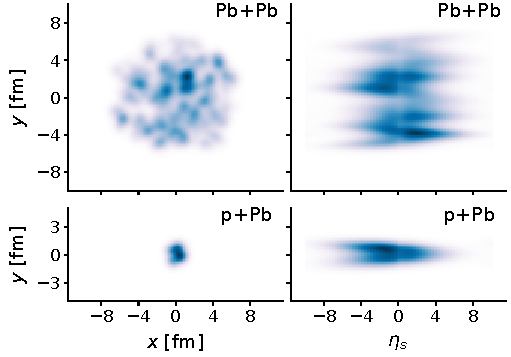
\includegraphics{trento3d/trento3d_example}
\caption{Initial entropy density in sample Pb+Pb (upper) and p+Pb (lower) events for cross sections of the $\eta=0$ and $x=0$ planes (left and right columns). Event is constructed using the relative skewness model in Table~\ref{tab:parametrization} with $\mu_0=1$, $\sigma_0=3$ and $\gamma_0=6$ along with midrapidity parameters from {Bernhard:2016tnd}.}
\label{fig:3d-example}
\end{figure}

\section{Reverse engineering the 3D initial condition}
In the final section of this chapter, I shall demonstrate applying both the hydrodynamic-based bulk simulation and the flexible \trento-3D initial condition to reverse engineer the 3D entropy deposition at the onset of hydrodynamics at the LHC energies.
Experimentally, one can only measure rapidity-dependent observables on an event averaged level, which already integrates the contribution of particle production over the transverse plane; while our parametrization in the \trento\ model only involves local functions of the participant density function.
Therefore, it is indeed a nontrivial task to infer the functional form of local entropy production $s(\x, \eta_s)$ from these ``global'' measurements.
The suitable statistical technique for parameter inference is the Bayesian 
analysis, which will be introduced in a great detail in chapter \ref{}.

\subsection{Sensitive observables to the initial entropy deposition}
\paragraph{The single particle spectra}
The most direct observable is the charged particle pseudo-rapidity density $\dnchdy$ measured for different collision systems and centralities.
The ALICE collaboration and the ATLAS collaboration has measured this quantity for both $Pb$-$Pb$ system ($-3.5<\eta<5.0$) and $p$-$Pb$ system ($|\eta| < 2.7$) {Abbas:2013bpa,ALICE:2015kda,Aad:2015zza}.
$\dnchdy$ can very well constrain the global rapidity profile and the centrality dependence of the mode, while the limitation being that it is less sensitive to the amount of longitudinal fluctuation.

\paragraph{Two particle pseudo-rapidity correlation}
A good probe of event-by-event longitudinal fluctuations is the two-particle pseudorapidity correlation observable $C(\eta_1, \eta_2)$,
\begin{eqnarray}
C(\eta_1, \eta_2) = \frac{ \left\langle N(\eta_1)N(\eta_2) \right\rangle}{\left\langle N(\eta_1)\right\rangle\left\langle N(\eta_2) \right\rangle}
\end{eqnarray}
The long range part of $C(\eta_1, \eta_2)$ can be shown to sensitive to initial state.
This is because correlation between particles separated by a large gap at proper time $\tau$ in rapidity can only come from proper time before $\tau e^{-|\eta_1-\eta_2|/2}$ even if the information travels at the speed of light.
For example, if one assumes the two particles separated by 4 units of rapidity are emitted at a constant $\tau = 8$ fm/$c$ hydrodynamic freeze-out hyper-surface and neglects the long range correlation that is built by the hadronic cascade, then any correlation must have come from before the proper time $ 8 e^{-2}\approx 1$ fm/c.

To see how $C(\eta_1, \eta_2)$ is related to the longitudinal fluctuation of the entropy deposition / particle production, we follow the analysis in  {Bzdak:2012tp, Jia:2015jga, ATLAS:2015kla} to decompose $\dnchdy$ for each event in a finite pseudo-rapidity window $[-Y, Y]$ using the normalized Legendre polynomials basis,
\begin{eqnarray}
T_n(x) &=& \sqrt{n + \frac{1}{2}} P_n(x)
\end{eqnarray}
And the event-wise charged particle distribution is then,
\begin{eqnarray}
\frac{dN}{d\eta} &=& \biggl\langle\frac{dN}{d\eta}\biggr\rangle \biggl[1 + \sum_{n=0}^\infty a_n T_n\left(\frac{\eta}{Y}\right) \biggr]
\end{eqnarray}
Where $\biggl\langle\frac{dN}{d\eta}\biggr\rangle$ is the reference multiplicity at mid-rapidity for an ensemble of events.
$a_0$ is the total multiplicity fluctuation and $a_1$ controls how the multiplicity distribution is tilted in rapidity in each event and so on.
Two-particle correlation $C(\eta_1, \eta_2)$ measures the variance of these $a_n$ coefficients.
Define the normalized event-wise distribution $R(\eta) = dN/d\eta /\langle dN/d\eta\rangle$, then the two particle correlations can be expressed as the event averaged products of $R$.
\begin{eqnarray}
C(\eta_1, \eta_2) &=& \left\langle R(\eta_1) R(\eta_2)\right\rangle \\
&=& 1 + \sum_{m, n}\langle a_m a_n\rangle  T_{mn}(\eta_1, \eta_2)
\end{eqnarray}
with $T_{mn}$ defined as,
\begin{eqnarray}
T_{mn}(\eta_1, \eta_2) &=& \frac{T_n(\eta_1)T_m(\eta_2) + T_m(\eta_1)T_n(\eta_2)}{2}.
\end{eqnarray}
Therefore, $
\langle a_m a_n\rangle$ can be extracted from two particle correlation.
Combinations like $\langle a_0 a_n\rangle$ reflects how the event-wise rapidity fluctuation correlates with multiplicity fluctuation, which can is canceled to first order by another normalization and define,
\begin{eqnarray}
 C_N(\eta_1, \eta_2) &= \frac{C(\eta_1, \eta_2)}{C_1(\eta_1)C_2(\eta_2)}\\
\end{eqnarray}
with the marginalized function,
\begin{eqnarray}
C_{1,2}(\eta_{1,2}) &= \int_{-Y}^{Y}C(\eta_1, \eta_2)\frac{d\eta_{2,1}}{2Y}.
\end{eqnarray}
And $C_N$ is directly related to the rapidity fluctuation of particle production,
\begin{eqnarray}
C_N(\eta_1, \eta_2) \sim 1 + \frac{3}{2}\langle a_1 ^2 \rangle \frac{\eta_1\eta_2}{Y^2} + \cdots.
\end{eqnarray}
and we shall focus on the $\langle a_1 ^2 \rangle$, which quantifies the amount of linearly-tilting fluctuation.

In additional to the initial condition fluctuation, short range correlation also contributes to the $a_1$ fluctuation {Denicol:2015bnf, Monnai:2015sca}.
The UrQMD hadronic afterburner is able to model certain type short range correlation coming from resonance decay and collisions, but jet-like correlations is hard to accounted for.

\subsection{Calibration of the 3D initial condition parameters}
The degrees of freedom of the initial condition model are,
\begin{itemize}[itemsep=0pt]
  \item[1--2.] Two normalization factors for Pb+Pb and p+Pb collisions at $\sqrts=2.76$~TeV and 5.02~TeV beam energies. they are not fully independent as the $N_{\textrm{p+Pb}} > N_{\textrm{Pb+Pb}}$ is always imposed in the parameter sweep because one expected more particle production is associated to the same thickness function at higher center-of-mass energy.
  \item[3.] The generalized mean parameter $p$ which modulates entropy deposition at midrapidity,
  \item[4.] A gamma shape parameter $k$, which controls the variance of proton-proton multiplicity fluctuations,
  \item[5.] A Gaussian nucleon width $w$, which determines initial state granularity;
  \item[6--8.] Three coefficients which modulate the local rapidity distribution's shift $\mu_0$, width $\sigma_0$, and skewness $\gamma_0$,
  \item[9.] A Jacobian factor $J$ for the conversion from rapidity to pseudorapidity.
\end{itemize}
And the range of the parameters is shown in \ref{tab:trento:parameters}.
One may notice that we did not use different width parameters for the rapidity distribution $\sigma_0$ for $Pb$+$Pb$ and $p$+$Pb$ collisions, though there are different beam energy.
We made this simplification because the the beam rapidity changes less than $8\%$ from $2.76$ TeV to $5.02$ TeV.

\begin{table}
\centering
\caption{Three-dimensional initial condition parameters}
\label{tab:trento:parameters}.
\begin{tabular}{lll}
      Parameter & Description	& Range \\
      \paddedhline
      $N_{\textrm{p+Pb}}$    & Overall p+Pb normalization      & 140.0--190.0 \\
      $N_{\textrm{Pb+Pb}}$   & Overall Pb+Pb normalization     & 150.0--200.0  \\
      $p$	                   & Generalized mean parameter      & -0.3--0.3 (with a prior)  \\
      $k$	                   & Multiplicity fluct.\ shape      & 1.0--5.0  \\
      $w$	                   & Gaussian nucleon width     & 0.4--0.6  \\
      $\mu_0$                & Rapidity shift mean coeff.\     & 0.0--1.0  \\
      $\sigma_0$             & Rapidity width std.\ coeff.\    & 2.0--4.0  \\
      \multirow{2}{*}{$\gamma_0$}             & \multirow{2}{*}{Rapidity skewness coeff.\ }      & 0.0--10.0 (rel) \\
                  &        & 0.0--3.6 (abs)  \\
      $J$	                   & Pseudorapidity Jacobian param.  & 0.6--0.9
\end{tabular}  
\end{table}

The dynamical model consists of both a 3+1D relativistic hydrodynamics and the hadronic afterburner.
The equation-of-state (EoS) is obtained by interpolating a state-of-the-art lattice-QCD EoS {Bazavov:2014pvz} at high temperature (zero baryon density) to a hadron resonance gas EoS at low temperature.
The energy density at which hydrodynamic energy momentum tensor is particulized into hadrons is $\epsilon_{sw} = 0.322$~GeV/fm$^3$ corresponding to a switching temperature close to the pseudo-critical temperature $T_{sw} \sim T_c = 0.154$~GeV).
As a remark, the relativistic hydrodynamics code \mbox{vHLLE} {Karpenko:2013wva} includes the viscous correction, bu we used its ideal mode in the parameter extraction.
This is because the parameter optimization process requires generating running the model on order hundreds different parameter sets.
For each parameter set, thoudands of minimum-biased events needed to be gerenated to achieve a good control of the statistical fluctuation, especially for the correlation observable. 
The full 3+1D viscous hydrodynamics is extremely time consuming, therefore we choose to ran the hydrodynamic model in its ideal mode and on a rather coarse grid.
While the justification is that the rapidity distribution of the multiplicity and normalized two-particle correlations is less sensitive to the viscous effect.
In the end, as a validation to this procedure, we will be using a set of high-likelihood parameter set and run the dynamical model with the viscous correction to see if other observables such as the harmonic flow, and event-plane decorrelations can be reasonably described.

\begin{figure}
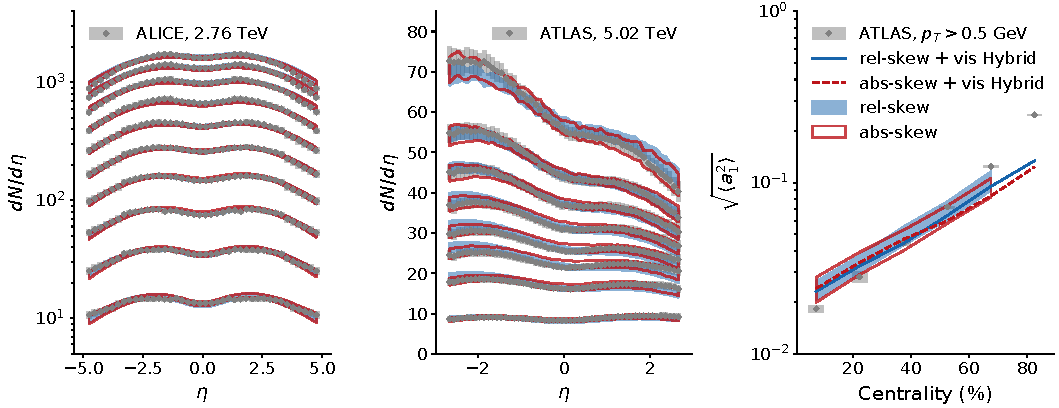
\includegraphics[width=\textwidth]{trento3d/post_obs.pdf}
\caption{}
\label{fig:trento:post_obs}
\end{figure}

Eventually, four thousands $Pb$+$Pb$ and ten thousands $p$+$Pb$ events are generated at $100$ set of parameter sets.
The computed $\dnchdy$ and $a_1$ fluctuation are computed at different centrality, and then the Bayesian analysis makes inference on the probability distribution on the parameters by comparing to measurements.
After the parameter calibration, the $\dnchdy$ and $a_1$ fluctuation as function of centrality is compared to measurements in figure \ref{fig:trento:post_obs}.
We found the single particle distribution can be well reproduced by the calibrated initial condition plus dynamical evolution, while the correlation observables can be described upto 50\% centrality. 
For more peripheral $Pb$+$Pb$ collisions, the hydrodynamical based model significantly underestimate the $a_1$ fluctuation.
We understand this as the consequence of inadequate modeling of the short range correlation for peripheral collisions, as these contributions becomes more important when the multiplicity is small ($\dnchdy\sim 250$ and $N_{\textrm{part}} \sim 75$ at 50\% centrality).
In fact, the authors of {ATLAS:2015kla} compared the measurements to the \mbox{HIJING} event generator that is based on mini-jet production.
It is found that these jet-like correlations agrees well with the $a_1$ fluctuation for peripheral collisions with $N_{\textrm{part}} \lesssim 80$, while it overshoots the data for more central collision.
The hydrodynamic model and mini-jet production model may need to be combined to fully understand the rms $a_1$, that at larger centrality, mini-jet production dominates the fluctuation of the $\dnchdy$, while as multiplicity increases and the final state interactions becomes more frequent, the short range correlation is diluted and the event-by-event asymmetry in the single-particle distribution dominates rms $a_1$.

\begin{figure}
\centering
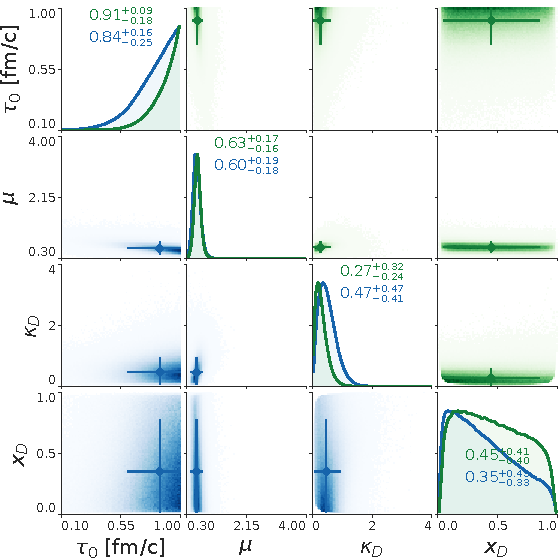
\includegraphics[width=\textwidth]{trento3d/posterior.pdf}
\caption{Posterior distributions of the model parameters, listed in Table~\ref{tab:parameters}, for the relative-skewness (blue lower diagonal) and absolute-skewness (red upper diagonal) models. The diagonal panels are the marginal likelihood distributions of individual model parameters, while off-diagonal panels are joint distributions for pairs of model parameters.}
\label{fig:trento:posterior}
\end{figure}

Regarding the performances of different parametrization of the skewness (``relative'' and ``absolute'' skewness), the ``relative'' skewness one does better in reproducing the uprising trend of rms $a_1$, while the absolute skewness one better describes the large $dnchdy$ asymmetry in the top 1\% $p$+$Pb$ collisions.
However, there is no strong evidence to favor any of them over the other.
We will see later that this is because the two parametrizations, though take different forms, actually results in a similar function form of $ds/d\eta(\eta; T_A, T_B)$ for typical values of $T_A$ and $T_B$ of a heavy nuclei.

\begin{figure}
\centering
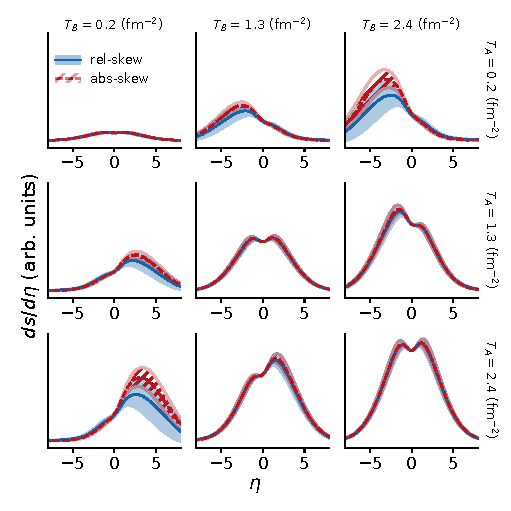
\includegraphics[width=.8\textwidth]{trento3d/post_dsdy}
\caption{Applying parameters sampled from the posterior probability distribution to Eq.~\eqref{cgf} along with Eq.~\eqref{regulateEq}, this plot shows the resulting local entropy profile $ds/d\eta$ varying $T_A$ and $T_B$ from $0.2~\text{fm}^{-2}$ to $2.6~\text{fm}^{-2}$. The lines are the mean predictions and the bands denote $1\sigma$ model uncertainties.
}
\label{fig:trento:post_dsdy}
\end{figure}

Looking at the posterior distribution of the parameters in figure \ref{fig:trento:posterior}, where the red and blue lines and color map corresponds to the parameter distribution of the ``absolute'' and ``relative'' skewness respectively.
One found that for the normalization parameters $N_{\textrm{PbPb}}$ and $N_{\textrm{pPb}}$, mid-rapidity entropy deposition parameter $p$, nucleon thickness function fluctuation parameter $k$, the width of the rapidity distribution $\sigma_0$ and the effective Jacobian $J$ have similar probability distributions between the two parametrizations.
However, the distribution of the asymmetry related parameters $\mu_0$ and $\gamma_0$ (anti-correlated) are very different between the two.
This is because the Bayesian calibration looks for the high-likelihood region of the parameter space to explain the data, and the two different prarametrizations can achieve this same goal by optimizing the parameter combinations differently.
For the ``relative'' skewness one, this is the region where a small shift of the mean $\mu$ and a large skewness $\gamma$; for the ``absolute'' skewness one, it corresponds to the region with a large $\mu$ but vanishing $\gamma$.
This does not mean that there are ``two models'' explaining the same data, because both of them are an oversimplified parametrization of $ds/d\eta(\eta; T_A, T_B)$ with infinitely many degrees of freedom. 
Instead, we should treat them as an estimation of the systematic uncertainty in extracting the function form of the initial 3D entropy deposition $ds/d\eta(\eta; T_A(\x), T_B(\x))$.
Therefore, it is more instructive to see the probability distribution of $ds/d\eta$ it self, given different values of $T_A(\x)$ and $T_B(\x)$.
In Fig.~\ref{fig:trento:post_dsdy}, we samples the calibrated parameter distributions and use them to draw the entropy density as function of rapidity at different values of $T_A$ and $T_B$. 
Again, the red and blue colors represents ``absolute'' and ``relative'' skewness parametrizations; the lines shows the median prediction and the bands are one standard deviation uncertainties. 
In each row and each column, $T_A$ and $T_B$ varies from $0.2~\text{fm}^{-2}$ to $2.4~\text{fm}^{-2}$. 
For references, the value of the thickness function at the center of a Gaussian proton with nucleon width $0.5$ fm is about $0.6~\text{fm}^{-2}$ and $T_{A,B} = 0.2~\text{fm}^{-2}$ corresponds to a nucleon's thickness at  1.5 width away from its center; while the maximum nuclear thickness function of a Pb nucleus is only about $2.2~\text{fm}^{-2}$.
Therefore, the chosen range of $T_{A,B}$ already cover the typical ranges and combinations for entropy production in a realistic heavy-ion collision.
One observe that the functional form of the $ds/dy$ between the two parametrization agrees within one standard deviation, with the deviations increases as the asymmetry increases.
Certainly, with a sufficient different $T_A$ and $T_B$ combination, the two results will have totally different predictions; however, within the physical range of the thickness function, the two methods converges on a similar behavior,
We conclude that by applying the hydrodynamic-based model and a flexible 3D initial condition, the form of the local rapidity distribution as function of the incoming participant densities can be reverse engineered using single particle pseudo-rapidity distribution and two-particle pseudo-rapidity correlation.

\subsection{Prediction with the calibrated 3D initial condition}
The calibrated initial condition is useful in predicting other rapidity-dependent observables.
Especially, because we have only used multiplicities observables $dnchdy$ and rms $a_1$ in the calibration, a prediction of azimuthal anisotropy related observables would provide an important validation of the initial condition.
We choose a set of high-likelihood parameters showed in table \ref{tab:chosen_parameters}.
The selected validation / prediction observables are pseudo-rapidity dependent harmonic flows, event-plane decorrelations and the symmetric cumulants which quantifies the correlation between different flow harmonics.

\begin{table}
\centering
\caption{A high likelihood parameter set}
\begin{tabular}{lll}
\hline
Parameter & rel-skew	& abs-skew \\
\hline
$N_{\textrm{Pb+Pb}}$   & 150.0     & 154.0  \\
$p$	    & 0.0      & 0.0  \\
$k$	    & 2.0     & 2.0  \\
$w$	    & 0.59     & 0.42  \\
$\mu_0$   & 0.0     & 0.75  \\
$\sigma_0$ & 2.9    & 2.9  \\
$\gamma_0$ & 7.3		& 1.0	\\
$J$	     & 0.75 & 0.75	\\
\hline
\end{tabular}
\label{tab:chosen_parameters}    
\end{table}

The elliptic and triangular flow from two-particle correlation $v_2\{2\}$ and $v_3\{2\}$ are calculated at as function of centrality at mid-rapidity (figure \ref{fig:trento:vn_cen}) and as function of pesudo-rapidity at different centrality (figure \ref{fig:trento:vn_eta}).
The first comparison is just to verify that with the inclusion of the longitudinal dependence, we are still able to describe flow measurement at mid-rapidity with a shear viscosity $\eta/s = 0.17 -- 0.19$ close to other phenomenological studies, though the bulk viscosity is not include.
The resultant calculation agrees with ALICE measurement within $\pm 10\%$ {Adam:2016izf}.

\begin{figure}
\centering
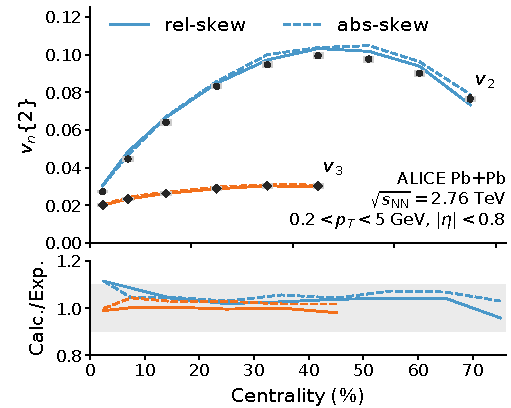
\includegraphics[width=.7\textwidth]{trento3d/vn_cen}
\caption{Elliptic and triangular flow cumulants $v_2\{2\}$ and $v_3\{2\}$ as a function of centrality calculated from 3+1D hybrid model simulations using constant specific shear viscosity $\eta/s=0.17$ and $0.19$ for relative- and absolute-skewness models respectively, zero bulk viscosity $\zeta/s=0$ and hydro-to-micro switching temperature $T_\text{sw}=154$~MeV.
The initial condition parameters are selected from the Bayesian posterior.}
\label{fig:trento:vn_cen}
\end{figure}

For the rapidity dependent flow figure \ref{fig:trento:vn_eta}, we used a larger $\eta/s=0.25--0.28$. 
This inconsistency is because the ALICE measurement extrapolate $p_T$ range for the rapidity-dependent flow down to 0, while the mid-rapidity  $p_T$ cut is $0.2 < p_T < 5.0$ GeV.
It would not be a problem for the model to describe both with the same transport parameters, if the $p_T$ differential flow and $p_T$ differential particle spectra are both reproduced.
However, due to the lack of a systematic tuning of the model parameters, including both shear and bulk viscosity, the current mean $p_T$ is too high.
Therefore, agreement with the $p_T$-integrated flow in one kinematic cut does not guarantee the agreement at $\eta=0$ to measurements that extrapolate to $p_T = 0$.
Since our primary interest is the $\eta$-dependence of the flow, we have chosen this larger-than-usual shear viscosity to match the $v_2{2}(\eta=0)$ values to data.
The calculated $v_2\{2\}$, $v_3\{2\}$, and $v_2\{4\}$ gradually decreases from mid-rapidity to forward / backward rapidity, which is also the trend of the data.
The shape of $v_3\{2\}$ is well described; but for $v_2\{2\}$ and $v_2\{4\}$ in the region $|\eta| > 2.0$, the data decreases much faster than our predictions.
There could be several reasons for this differences.
For example, $v_3$ are driven by fluctuations while $v_2$ is driven by a combination of both collision geometry and fluctuations. It is possible that the current initial condition model produce enough amount of fluctuation, but inadequate variance of the the overlapping geometry as function of space-time rapidity.
It is also showed in a study of at RHIC energies {Denicol:2015bnf} that the decreasing slope of $v_n(\eta)$ can be sensitive to the shear viscosity in the hadronic phase. 
But in our model, the transport properties of the system below $T_c$ is all encoded in UrQMD and is not tunable. 
Moreover, we have assumed that hydrodynamization happens at a constant proper time hypersurface. 
While it is possible a constant entropy density hypersurface is a better criteria, and as a result the matter at larger rapidity experiences less pressure driven expansion.
To systematically investigate all these effects, a future global parameter calibration including both initial condition parameters, transport parameters, and matching parameters is inevitable and is also feasible given the advance of the dynamical models and programming developments as well as more powerful computing resources.


\begin{figure}
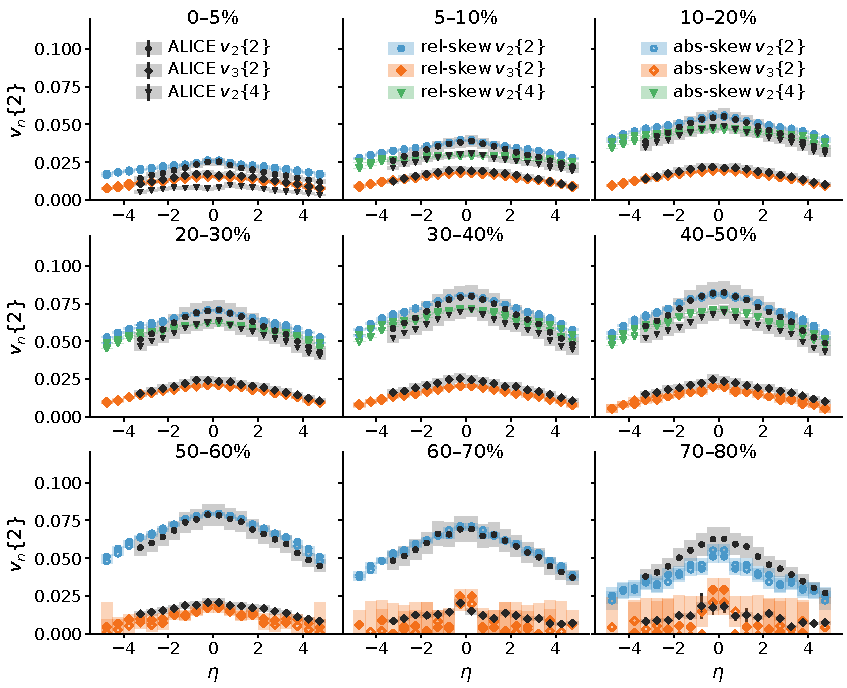
\includegraphics[width=\textwidth]{trento3d/vn_eta}
\caption{Pseudorapidity dependence of anisotropic flow coefficients $v_2\{2\}$, $v_3\{2\}$ and $v_2\{4\}$ (blue circle, green triangle and orange diamond shaped symbols) calculated from the hybrid model with constant specific shear viscosity $\eta/s=0.25$ and $0.28$ for relative- and absolute-skewness models respectively (solid and open symbols), compared to data from ALICE (smaller black symbols) with $p_T > 0$~GeV (extrapolated) in different centrality bins. 
The bands for each theory calculation point indicate $1\sigma$ statistical error, while experimental bands/bars denote $1\sigma$ systematic and statistical errors respectively.}
\label{fig:trento:vn_eta}
\end{figure}

The event-plane decorrelation reveals longitudinal structure of the event from a different angle, by quantifying how much the event-plane angles,
\begin{eqnarray}
\Psi_n^\text{EP} = \frac{\text{atan2}(\langle \sin n \phi \rangle, \langle\cos n \phi \rangle)}{n},
\end{eqnarray}
This event-plane decorrelation been studied using initial conditions from 3D extended Glauber model and A Multi-Phase Transport (AMPT) model {Bozek:2015bna,Jia:2014ysa, Xiao:2012uw,Pang:2015zrq}.
Recently developments such as solving the gluonic Yang-Mills dynamics in three-dimensions also studied the decorrelation of the initial eccentricity.
In our model, the geometry at forward and backward rapidity are dominated by the participants density of two different nuclei.
And in between, the entropy production smoothly transit from one to anther and so are the orientation of the energy density eccentricities that drives the flow of particles.
Phenomenological speaking, the decorrelation effect is important those observable that involves a large rapidity gap and should be corrected.
The CMS collaborations quantifies the decorrelation by a three-bins factorization ratio {Khachatryan:2015oea},
\begin{eqnarray}
r_n(\eta^a, \eta^b) &= \frac{V_{n\Delta}(-\eta^a, \eta^b)}{V_{n\Delta}(\eta^a, \eta^b)}, \\
V_{n\Delta}(\eta^a, \eta^b) &= \langle\langle \cos(n\Delta\phi) \rangle\rangle,
\end{eqnarray}
where the double average run over all particle pairs and all events.
The ratio is involves three rapidity bins one near $\eta^b$ and the other two near $\pm\eta^a$.
This ratio measures the decorrelation between two event planes separated by a larger rapidity gap $\eta^a + \eta^b$ relative to the decorrelation over a smaller gap $|\eta^a - \eta^b|$.
Experimentally, one would like the reference $\eta^b$ larger to surprises the short range correlations correlation, which produces signals that does not come from the single particle event-plane.
However, the way we build our model is to extend the mid-rapidity entropy deposition to finite rapidity, and this extension will eventually failed at sufficiently large rapidity because the model behavior at those part is not well constrained.

In figure \ref{fig:trento:epd}, we compare the model calculations to data with both a large $4.4<\eta^b<5.0$ (right) and a relative smaller $3.0 < \eta^b< 4.0$ (left).
The predicted factoziation ratios decreases linearly with the the increasing rapidity gap.
Using reference particles from $3.0 < \eta^b< 4.0$, the decorrelation is reproduced at larger centrality but not for central collisions.
Because the $n=2$ event-plane has a preferred direction defined by the impact parameter, while $n=3$ event-plane does not, we observe that $n=2$ factorization ratio decorrelates slower than the $n=3$ ratio, except for the most central collision when $n=2$ event-plane is also dominated by fluctuations.
Comparing to data with reference particle from $4.4<\eta^b<5.0$, the experimental data stays similar to the the previous case except for central collisions, but the prediction is completely off.
This is simply because the model fails on the details at large rapidity as we explained earlier.
Given the present comparison, we conclude that the valid range of the model is $|\eta| < 4.0$.

\begin{figure}
\centering
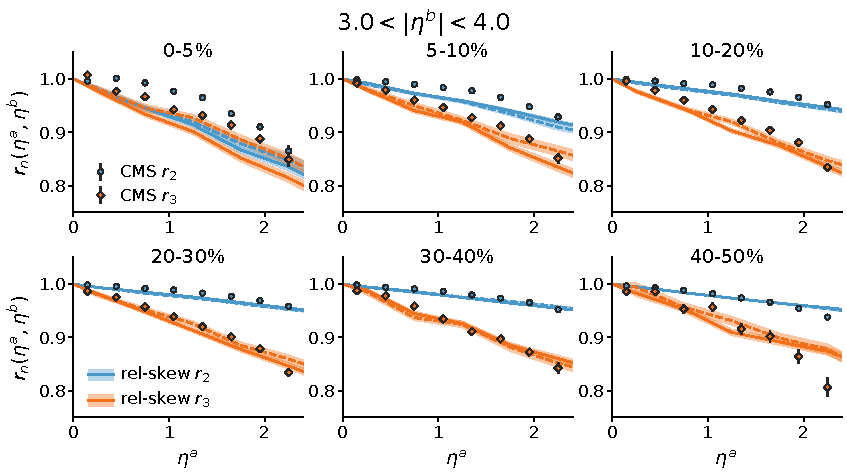
\includegraphics[width=.495\textwidth]{trento3d/evt_pln_decorr_near}
\hfill
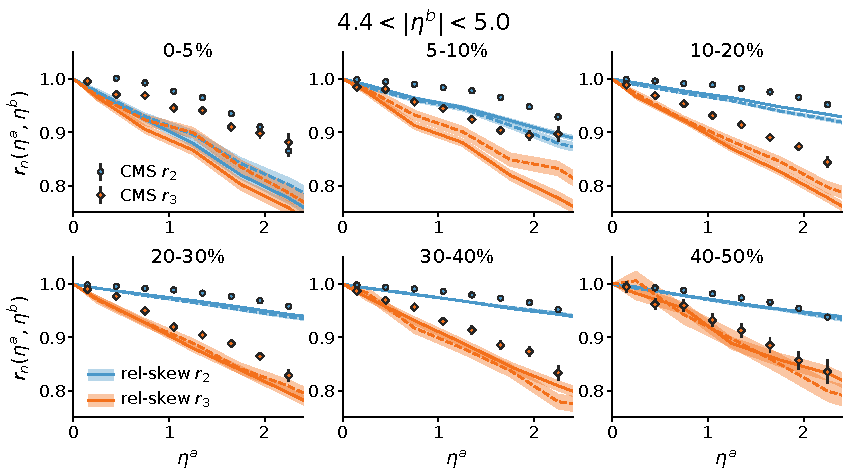
\includegraphics[width=.495\textwidth]{trento3d/evt_pln_decorr_far}
\caption{Left: The event-plane decorrelation for $n=2,3$ in different centrality bins with the reference particles from $3.0<|\eta^b|<4.0$.
  Right: The same quantities as the left panel but with the reference particles from $4.4<|\eta^b|<5.0$. 
  Theory bands indicate $1\sigma$ statistical error, while experimental bands/bars denote $1\sigma$ systematic and statistical errors respectively.}
\label{fig:trento:epd}
\end{figure}

The last observable is an intricate one that measure how different order of flow harmonics correlated with each other.
Methods such as event-shape engineering and multi-particle symmetric cumulants are used to extract these information {Schukraft:2012ah, Aad:2015lwa, Bilandzic:2013kga}.
ALICE experiments adopt the symmetric cumulants $SC$ method {ALICE:2016kpq}.
It is a four particle correlation involves two different harmonic orders $m$ and $n$
\begin{eqnarray}
SC(m, n) &=& \langle\langle \cos(m\phi_1+n\phi_2-m\phi_3-n\phi_4)\rangle\rangle \nonumber \\
\nonumber &-& \langle\langle\cos[m(\phi_1-\phi_2)]\rangle\rangle\langle\langle\cos[n(\phi_1-\phi_2)]\rangle\rangle \label{eq:scmn}\\
&=& \langle v_m^2 v_n^2 \rangle - \langle v_m^2\rangle\langle v_n^2\rangle.
\end{eqnarray}
It is clear from the second equation that it measures the covariance between $v_n^2$ and $v_m^2$.
One can also define the normalized symmetric cumulants (NSC),
\begin{equation}
NSC(m,n) = \frac{SC(m,n)}{\langle v_m^2\rangle\langle v_n^2\rangle}.
\end{equation}
These observables are interesting because they are robust against now-flow effects, and have been shown to be sensitive to the temperature dependece of the transport coefficients {Niemi:2012aj}.
Other analysis show that $SC(4,2)$ probes the non-linear response of the hydrodynamic evolution, while $SC(3,2)$ is more sensitive to initial conditions {Zhu:2016puf}, etc.

The relative- and absolute-skewness calculations are arranged on the left and right of \ref{fig:trento:smn}. Symmetric cumulants $SC(4,2)$ (blue) and $SC(3,2)$ (green) are displayed in the top plots, and $NSC(4,2)$ (blue) and $NSC(3,2)$ (green) in the bottom plots.
Within each plot, black dots are ALICE measurements at midrapidity $|\eta|<0.8$, which should be compared to the calculation shown in solid lines.
The calculation shown in dashed lines are our predictions at forward/backward rapidity $2.5 < |\eta| < 3.5$ using,
\begin{eqnarray}
SC^\prime(m, n) &=& \langle\langle \cos(m\phi_1+n\phi_2-m\phi_3^\prime-n\phi_4^\prime)\rangle\rangle \\
\nonumber &-& \langle\langle\cos[m(\phi_1-\phi_2^\prime)]\rangle\rangle\langle\langle\cos[n(\phi_1-\phi_2^\prime)]\rangle\rangle, \label{eq:scmn}
\end{eqnarray}
where the two of the particles (primed) are selected from the forward/backward rapidity bins, while the rest of the two still come from the mid-rapidity bin  $|\eta|<0.8$.

At mid-rapidity, the calculated (normalized) symmetric cumulents reproduce the trend of the measurements, and the ``relative'' skewed initial condition does a better quantitative job than the ``absolute'' skewed model.
At forward and backward rapidity, though the magnitudes of both $SC(m,n)$ and $v_n$, $v_m$ changed, the normalized symmetric cumulants remains the same as the one at mid-rapidity.
This is a prediction that can be checked in future measurements to put further constraints on the three-dimensional initial condition model.

\begin{figure}
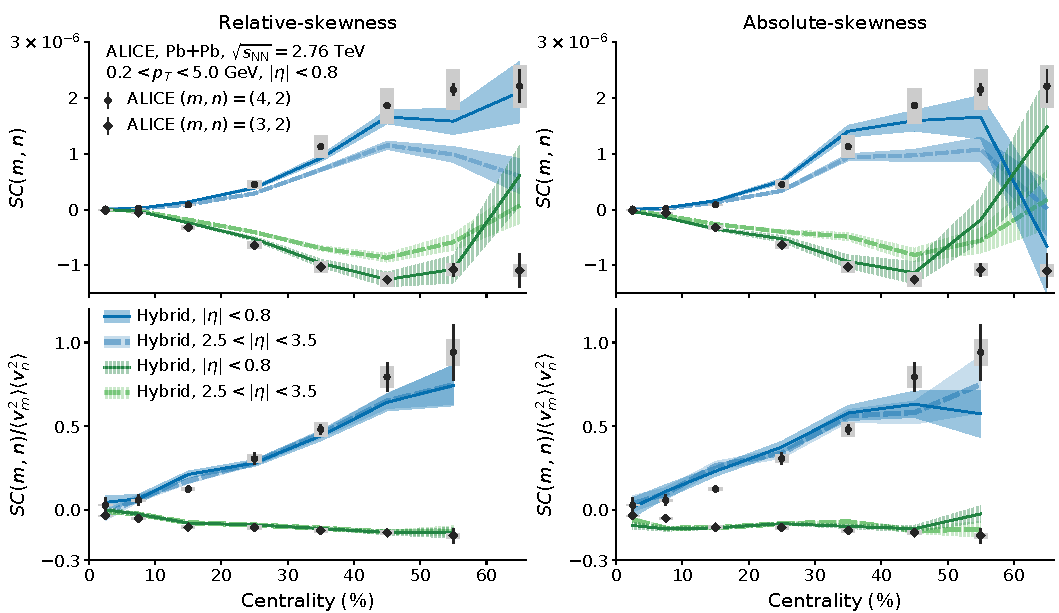
\includegraphics[width=\textwidth]{trento3d/smn}
\caption{Top row: calculated $SC(4,2)$ and $SC(3,2)$ as functions of centrality compared to ALICE measurements, with the same 3D hybrid model set-up as used for Fig. \ref{fig:vn_cen}.
  We conduct calculations in two kinematic ranges: $|\eta|<0.8$ is the pseudorapidity cut used by current the ALICE measurement and $2.5<|\eta|<3.5$ is our prediction for the symmetric cumulants away from mid-rapidity in the Pb+Pb system.
  Bottom row: $SC(m,n)$ normalized by $\langle v_m^2\rangle\langle v_n^2\rangle$ for two two kinematic ranges.
  The left column and right column show results using relative- and absolute-skewness respectively.
}
\label{fig:trento:smn} 
\end{figure}

\section{Summary}
As a summary of this section, I have introduced the hydrodynamic-based  medium evolution model that is very successful in explaining a spectrum of different soft observables.
The sensitivity of the harmonic flows to the QCD transport coefficients allows one to a model parameter calibration using advanced statistical technique.
On the other hand, the initial condition for the dynamical model is still a large source of uncertainty in both data interpretation and parameter extraction.
The \trento\ initial condition model was developed as a flexible ansatz for mid-rapidity entropy / energy deposition so that the initial condition and interested transport coefficients can be calibrated simultaneously to data.
Finally, I discussed my work on extending the \trento\ initial condition to include rapidity dependence and the use of multiplicity observable to reverse-engineer the functional form of initial 3D entropy deposition.
The results can be used to predict more rapidity-dependent observables, which is useful to study the medium dynamics in a hydrodynamic approach at large rapidity.
With the current accuracy, not all observables are reproduced to a similar level of accuracy as the mid-rapidity case.
This is partly due to the simplicity of the modeling, as well as the lack of global fit of all parameters including both 3D initial conditions and transport coefficients.
This is an important practice in the future to study how far can one push the application of hydrodynamics into the large rapidity region and how the inclusion of longitudinal fluctuation affects the extracted QCD transport coefficients.